\documentclass{article}
\usepackage{tikz}
\begin{document}    
    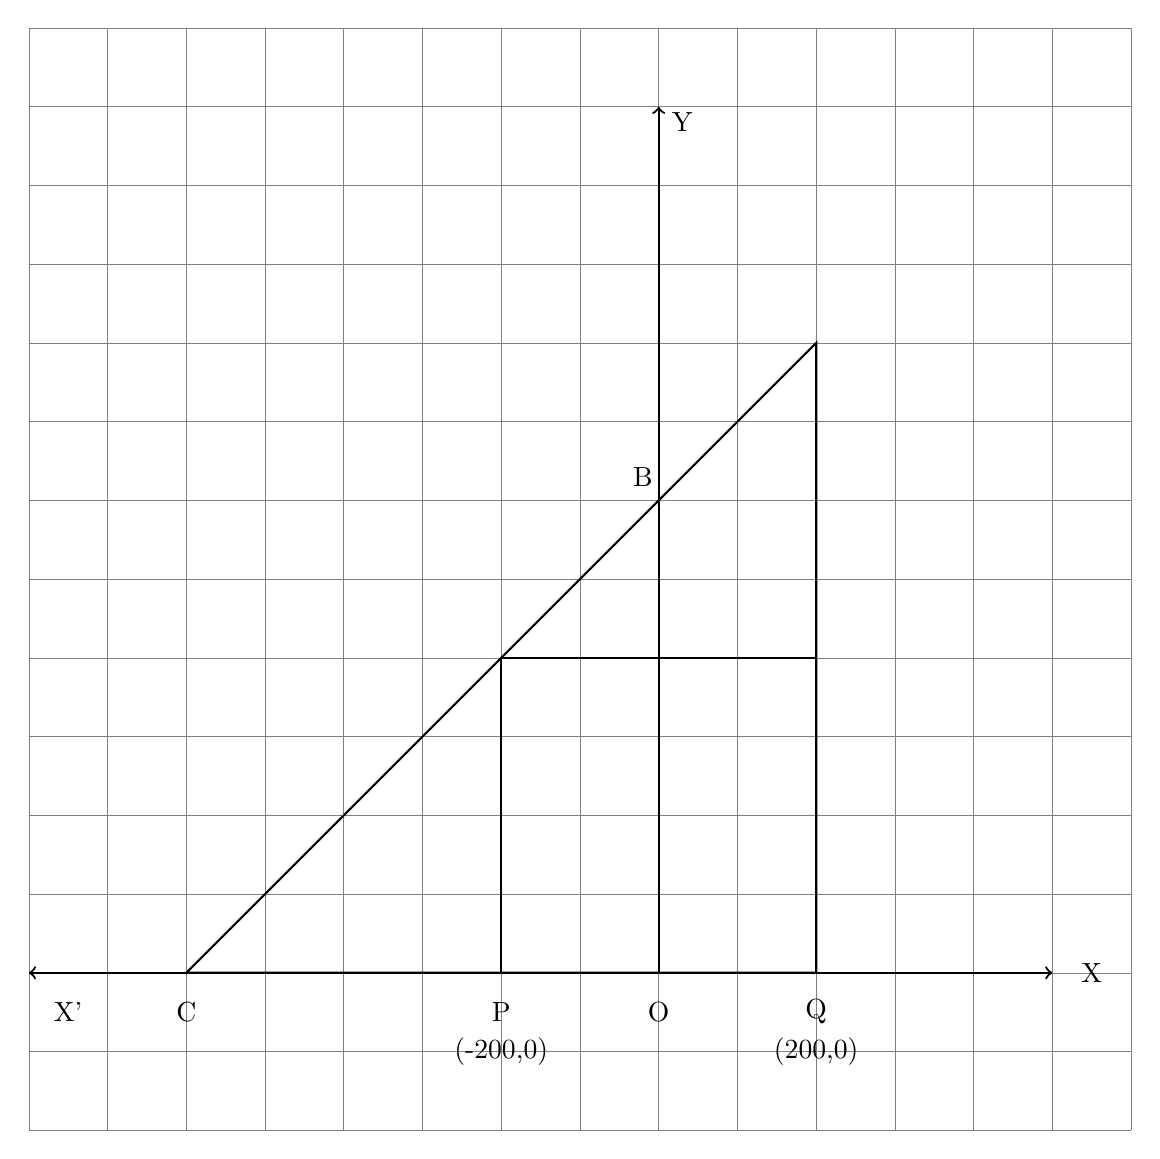
\begin{tikzpicture}
    \draw[help lines] (0,0) grid (14,14);
    \draw[<->, thick] (0,2)--(2,2)--(13,2);
    \draw[->, thick] (8,2)--(8,13);
    \draw[thick] (6,2)--(6,6)--(10,6)--(10,2);
    \draw[thick] (2,2)--(10,2)--(10,10)--(2,2);
    \node at (13.5,2) {X};
    \node at (2,1.5) {C};
    \node at (6,1.5) {P};
    \node at (8,1.5) {O};
    \node at (7.8,8.3) {B};
    \node at (8.3,12.8) {Y};
    \node at (6,1) {(-200,0)};
    \node at (10,1.5) {Q};
    \node at (10,1) {(200,0)};
    \node at (0.5,1.5) {X'};
    \end{tikzpicture}
\end{document}
